% Capítulo 4
\chapter{Fundamentação Teórica}\label{cap:fundamentacao-teorica}

Este capítulo está organizado para introduzir os conceitos-chave e explicar detalhadamente cada seção. Serão apresentados os fundamentos teóricos que sustentam o desenvolvimento e a aplicação de dois modelos fundamentais para a implementação da proposta: o modelo cognitivo e o modelo de template multicamadas para geração automática de questões. Cada subseção abordará os conceitos essenciais relacionados a esses modelos, detalhando suas características, funcionamento e contribuições para o objetivo final do estudo.

\section{Modelo Cognitivo}
A construção de questões em larga escala, por meio de processos automatizados, tem-se tornado uma prática cada vez mais relevante na área de avaliações educacionais. Nesse contexto, a elaboração de um modelo cognitivo sólido constitui um passo fundamental para embasar a Geração Automática de Questões (\gls{aig}). De modo geral, modelos cognitivos podem ser definidos como descrições explícitas de como os estudantes processam informações e resolvem tarefas específicas, envolvendo as habilidades e os raciocínios que se espera que demonstrem em uma dada questão. O processo de construção desse modelo, conforme discutido por \parencite{gierl2021}, esta técnica consiste em identificar, organizar e documentar de forma sistematizada os conceitos, parâmetros e restrições que caracterizam tanto a criação de uma questão quanto a forma como os estudantes são esperados a resolvê-la.

A relevância do modelo cognitivo torna-se ainda mais evidente quando se busca a replicabilidade e a qualidade das questões geradas em larga escala. Esse detalhamento fornece a base para a elaboração dos templates, os quais orientam a criação de questões capazes de manter o mesmo nível de complexidade, exigência cognitiva e alinhamento ao conteúdo que se deseja avaliar. Dessa forma, o modelo cognitivo funciona como um roteiro que descreve tanto os conteúdos quanto a lógica da questão a ser gerada.

O modelo cognitivo é a base fundamental para a criação dos templates, pois organiza e descreve todos os elementos necessários para sua construção. Os templates, por sua vez, atuam como estruturas que convertem essas informações de forma efetiva, resultando em questões de avaliação individual claras e alinhadas aos objetivos de ensino.


\section{Estrutura do Modelo Cognitivo}

O modelo cognitivo funciona como um guia para organizar os elementos necessários para a construção dos templates. Estes templates servem como estruturas que traduzem as diretrizes estabelecidas no modelo cognitivo em questões, claras, consistentes e alinhadas aos objetivos educacionais \parencite{keehner2017, gierl2017}. Para garantir a qualidade e replicabilidade, o modelo cognitivo deve ser estruturado de maneira a detalhar os seguintes aspectos fundamentais : 

\subsection{Problemas e Cenários}

A primeira etapa do processo de construção do modelo cognitivo consiste em definir claramente o objetivo da avaliação, identificando o problema central que servirá de base. Em uma disciplina de algoritmos que aborda estruturas de repetição, podemos optar por explorar aspectos como o tipo de laço ou os componentes fundamentais de uma estrutura controlada por um contador. Dessa forma, podemos assegurar que as habilidades específicas a serem avaliadas estejam claramente refletidas na questão. E, posteriormente, elaborar possíveis cenários relacionados ao problema principal. Nas avaliações sobre estruturas de repetição, podemos incluir cenários que envolvam a identificação do tipo de laço utilizado em um trecho de código, a utilização de contadores para controlar iterações ou a aplicação de estruturas de repetição em situações práticas de desenvolvimento de algoritmos. Cada cenário amplia a diversidade das questões, mantendo a coerência com o objetivo da avaliação.

\subsection{Fontes de Informação}

As fontes de informação constituem o conjunto de conteúdos e matérias que podem abranger dados quantitativos, textos, fórmulas, diagramas, trechos de código, figuras ou qualquer outro elemento que possibilite aos estudantes acionarem os conhecimentos e habilidades que se deseja avaliar. Cada fonte de informação deve ser descrita de forma detalhada, de modo a estabelecer claramente a relação entre o conteúdo apresentado e as características a serem avaliadas.


\subsection{Características (\textit{Features})}

As características (\textit{features}) são atributos fundamentais que compõem as dimensões ou variáveis do modelo cognitivo. Elas definem os aspectos que podem ser ajustados na criação dos templates. Na prática,cada característica é composta por elementos, valores e restrições:


\subsection{Elementos}
Elementos representam as variações possíveis dentro de uma categoria ou dimensão específica da \textit{feature}, permitindo a manipulação do conteúdo através de componentes básicos que podem ser uma variável numérica, um trecho de código ou um termo técnico relevante para a questão. Os elementos devem ser construídos de forma a facilitar a combinação de um elemento com outro.

\subsection{Valores}
Valores são as possíveis combinações que os elementos podem assumir dentro de uma faixa de opções. Eles definem as variações quantitativas ou qualitativas que um elemento pode ter.

\subsection{Restrições}
Restrições são regras ou condições que limitam como os elementos e seus valores podem ser combinados. Elas garantem que as combinações resultantes sejam válidas, coerentes e alinhadas aos objetivos da questão, evitando a geração de questões inválidas ou sem sentido.

A figura a seguir apresenta a estrutura hierárquica do modelo cognitivo para geração automática de questões, destacando os principais componentes e suas inter-relações. Ela organiza os elementos em três níveis principais : problemas e cenários, fontes de informação e características (\textit{features}). Essa visualização facilita o entendimento do processo de construção do modelo cognitivo.


\begin{figure}[ht]
	\centering
	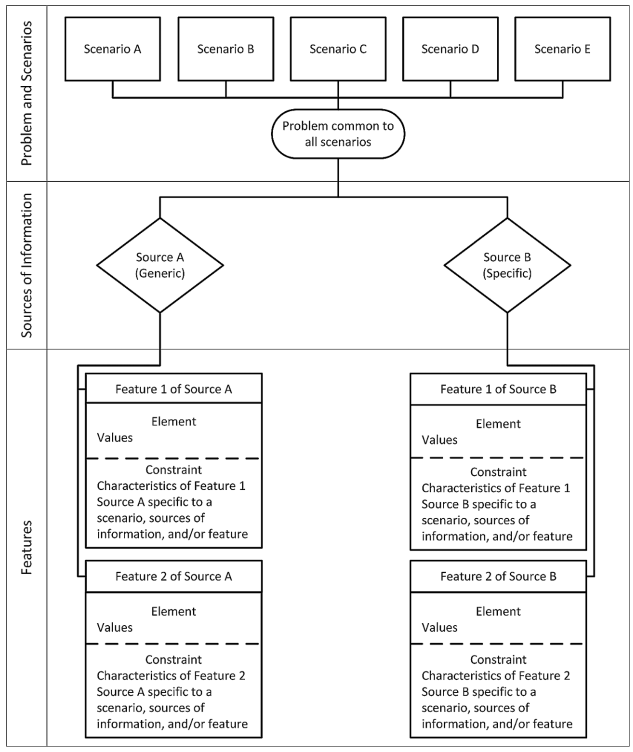
\includegraphics[width=14cm]{./imagens/capitulo4/cognitive-model}
	\caption{Estrutura do Modelo Cognitivo (Gierl, 2021)}
	\label{fig:cognitive-model}
\end{figure}

\section{Relação do Modelo Cognitiva e Construção de Templates }

O modelo cognitivo é a base fundamental para a criação dos templates, pois organiza e descreve todos os elementos necessários para sua construção. Os templates, que por sua vez, atuam como estruturas que convertem essas informações de forma efetiva, resultando em questões de avaliação individual claras e alinhadas aos objetivos de ensino.
\cite{gierl2016, gierl2017, keehner2017, gierlbulutzhang2018 }. É a partir desse modelo que se definem, de maneira estruturada, aspectos como:

\begin{itemize} \item Conteúdos a serem avaliados (conceitos, regras e relações); \item Habilidades e processos de pensamento esperados dos estudantes (como identificar, analisar, resolver problemas); \item Restrições e parâmetros de combinação (limites numéricos, coerência semântica, condições mínimas para a aplicação de um conceito). \end{itemize}





Por outro lado, os \textit{templates} são estruturas que convertem o modelo cognitivo em modelos práticos de questões \cite{gierl2024}. Cada \textit{template} especifica como as informações do modelo serão incorporadas ao enunciado e às alternativas (corretas e incorretas). Assim, a relação entre o modelo cognitivo e os \textit{templates} pode ser resumida nos seguintes pontos:

\begin{enumerate} \item \textbf{Definição de elementos básicos de uma questão:} O modelo cognitivo descreve quais componentes (por exemplo, dados quantitativos, termos-chave, situações-problema) precisam estar presentes para que o item seja relevante e alinhado aos objetivos pedagógicos. O \textit{template} organiza esses componentes em uma estrutura pronta para gerar diferentes versões de questão \cite{lane2016}.
\item \textbf{Combinação e manipulação de parâmetros:} Enquanto o modelo cognitivo define as regras de como os conteúdos e as habilidades podem ser combinados (por exemplo, valores ou conceitos que podem variar para alterar a dificuldade de um item), o \textit{template} coloca essas regras em prática. Em outras palavras, integra os diversos elementos para criar itens com diferentes níveis de complexidade, mantendo a coerência com a proposta original \cite{embretson2017}.

\item \textbf{Padronização e escalabilidade:} A adoção de um modelo cognitivo bem elaborado facilita a padronização do processo de elaboração de itens em grande escala. Como os \textit{templates} seguem o mesmo conjunto de regras e estruturas, as questões criadas tendem a manter consistência em termos de conteúdo, formato e nível de exigência cognitiva \cite{gierl2016, gierl2017}.

\item \textbf{Validação e ajustes contínuos:} Se um \textit{template} gerar um item que se revele muito fácil ou muito difícil, é possível identificar rapidamente se o problema está no modelo cognitivo ou no próprio \textit{template}, permitindo o ajuste da regra que originou a inconsistência. Dessa forma, a correção ocorre em nível conceitual (no modelo) ou técnico (na estrutura do \textit{template}), preservando a qualidade dos itens e mantendo-os alinhados aos propósitos da avaliação \cite{gierlbulutzhang2018}.
\end{enumerate}
Em síntese, o modelo cognitivo oferece a base teórica e estrutural, descrevendo de forma clara o que e por que está sendo avaliado, enquanto o \textit{template} representa a forma de aplicação prática dessas informações na formulação das questões \cite{gierl2024}. Essa integração torna a Geração Automática de Questões mais sólida, pois cada item criado segue a mesma lógica e mantém um padrão de qualidade, contribuindo para avaliações mais consistentes e confiáveis.

\section{Modelo de Template}

\subsubsection{Template 1-Layer}
\subsubsection{Template N-Layers}

